% DOCUMENT CLASS %
\documentclass[a4paper, 12pt]{article}   % for A4 Paper, 12pt fontsize.
\setcounter{tocdepth}{4}
\setcounter{secnumdepth}{3}

% PACKAGES%
\usepackage{amsfonts}   % For a basic mathfont (many will be replaced by stix)
\usepackage{amsmath}    % For basic math symbols
%\usepackage{bbm}        % For \mathbbm (better version of \mathbb)
\usepackage{mathrsfs}   % For \mathscr
\usepackage{hyperref}   % For footnotes
\usepackage{csquotes}   % For \textquote{}
\usepackage{IEEEtrantools}  % For better alignments
\usepackage{tikz}   % For a macro
\usepackage{listings} % For code
\usepackage{xcolor}   % For ... code
\usepackage[stretch=40]{microtype}
\usepackage{enumitem}
\usepackage{geometry}
\usepackage[color=gray]{todonotes}

% Language
\usepackage[english]{babel}

% If needed
\usepackage[nohyperlinks,smaller]{acronym}

% For tests
\usepackage{lipsum}

%%% ENVIRONMENTS %%%
\usepackage{amsthm}
\usepackage[nameinlink]{cleveref}

% Definition environment
\theoremstyle{definition}
\newtheorem{definition}{Definition}[section]
% Configure reference name
\crefname{definition}{Definition}{Definitions}

\theoremstyle{definition}
\newtheorem{exercise}{Exercise}[section]
\crefname{exercise}{Exercise}{Exercises}

\theoremstyle{definition}
\newtheorem{algorithm}{Algorithm}%[section]
\crefname{algorithm}{Algorithm}{Algorithms}

\theoremstyle{theorem}
\newtheorem{theorem}{Theorem}%[section]
\crefname{theorem}{Theorem}{Theorems}
%%%

%%% FONT CONFIGURATION %%%
\usepackage{fontspec}

% Updated version of Crimson Text
\setmainfont{Cochineal}
\setmonofont{Cascadia Code}[Scale=0.8]
\usepackage[cochineal]{newtxmath} % To use Cochineal as a Math Font
%%%

% MAKE DESCRIPTION ENVIRONMENTS HAVE ITALICIZED ITEMS %
\renewcommand{\descriptionlabel}[1]{\hspace{\labelsep}\textit{#1}}

% SETS %
\newcommand*{\R}{\mathbb R}    % Set of real numbers
\newcommand*{\N}{\mathbb N}    % Set of natural numbers
\newcommand*{\Z}{\mathbb Z}    % Set of integers
\newcommand*{\Q}{\mathbb Q}    % Set of rational numbers

% BASIC CONFIGURATION %
\pagestyle{plain}
\allowdisplaybreaks

% CODE %
\definecolor{codepurple}{HTML}{7f0055}
\definecolor{comment}{RGB}{0,128,0}
\definecolor{number}{RGB}{9,136,90}
\definecolor{string}{RGB}{163,21,21}

% Things that are the same in all styles
\lstdefinestyle{basic}{
    basicstyle=\ttfamily\footnotesize,
    breakatwhitespace=false,
    breaklines=true,
    frame=leftline,
    keepspaces=true,
    numbers=left,
    firstnumber=1,
    numbersep=5pt,
    showspaces=false,
    showstringspaces=false,
    showtabs=false,
    tabsize=2,
    commentstyle=\itshape\color{comment},
    stringstyle=\color{string},
    keywordstyle=\bfseries\color{codepurple},
    texcl=true,
    mathescape=true
}

\lstdefinestyle{default}{
    style=basic,
    language=c,
}

\lstset{style=default}

\title{Internet of Things and Wireless Networks}
\date{Summer Term 2026}
\author{Henri Heyden \\%
    \small stu240825 \\%
    \and%
    Parham Razaghian \\%
    \small stu258323%
}


\begin{document}
\maketitle

%\setcounter{section}{0}
%% Skip the first one
%\setcounter{exercise}{1}

\begin{exercise}[C Programming] \hfill
    \begin{itemize}
        \item[Q1] I've got a score of 7/10 points.

        \item[Q2] The stack is the memory portion which stores values whose longlivity is defined by the scope of the function it is defined in (inline blocks), and some information about the current function call tree, e.g., the callers registers.
            On function call the stack grows upward, on function return, the stack shrinks.
            Therefore, the programmer must not access any variables whose value is stored on the stack, after the execution leaves the scope it was declared in.

            This is different for heap-stored values, which the programmer has to manually allocate (assign an address and size) and deallocate.
            Again, the programmer must not access to any value whose address has been deallocated to ensure memory safety, as the portion may have been already allocated for a different process.

            When the stack grows too long, which can happen with, e.g., unrestricted recursive function calls, the process is forced to terminate, because the stack grew bigger, than its bounds.

        \item[Q3] The C \lstinline|static| keyword is different from the commonly associated concept of a \emph{static variable}, which has the same lifetime as the program.
            Instead, there are two main different meanings of the keyword, related to where a function or variable is declared.
            If a variable is declared with the storage modifier \lstinline|static| inside a function, it keeps its value between invocations, which is similarly to the referenced concept.
            If a variable is declared \lstinline|static| \emph{outside} any function, or a function is declared \lstinline|static|, access to the variable or function is only allowed to the scope of the file it is declared in.
            In this case, the variable or function is not accessible in external scopes.

        \item[Q4] You can write \lstinline|K/16| as \lstinline|K>>4|, and \lstinline|K%16| as \lstinline|(K>>4) & 0x1111|.
    \end{itemize}
\end{exercise}

\setcounter{exercise}{3}

\begin{exercise}[Running BLE Example in Renode] \hfill
    \begin{itemize}
        \item[Q5] See \autoref{fig:1}.
            While not included in the screenshot, Wireshark is also installed and able to capture Bluetooth and WLAN snippets.
    \end{itemize}

    \begin{figure}[b]
        \centering
        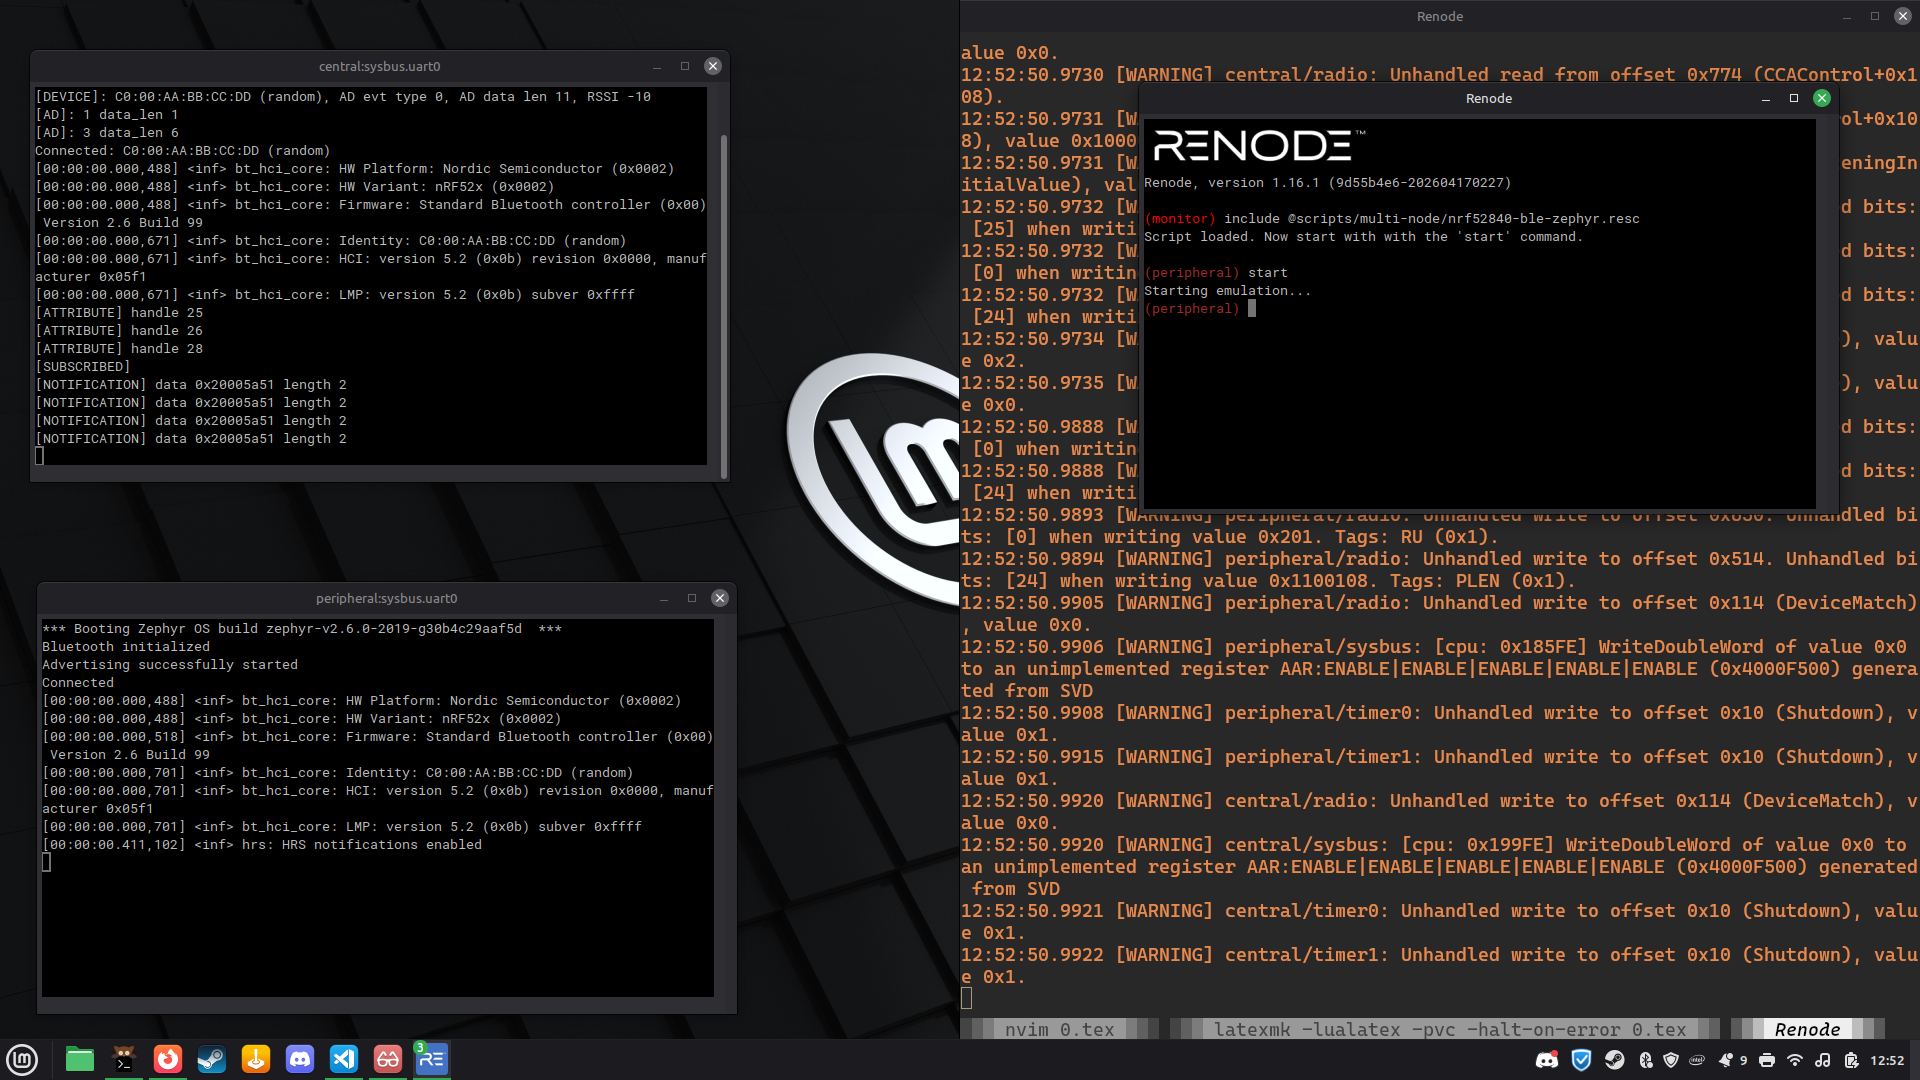
\includegraphics[width=0.6\textwidth]{./screenshot.png}
        \caption{Renode BLE demo running on Linux Mint.}
        \label{fig:1}
    \end{figure}
\end{exercise}

\begin{exercise}[Basic Networking] \hfill
    \begin{itemize}
        \item[Q6] A BLE simulation is configured in Renode by building Zephyr firmware with the desired tool, e.g, PlatformIO or west.
            The path to the generated firmware can be stored in a Renode shell variable for ease of use.
            Now we have to create a virtual device, link a platform description, e.g., nrf52840, and connect it to a medium, which serves as a simulated pathway between devices.
            Now for each device we must set it active and load the respective firmware.
            Finally we can start the simulation.
        \item[Q7] The advertiser tries to continuously broadcast \lstinline|"Hello IoT course!"|, while the scanner tries to receive these advertisements and print meta information about them.
        \item[Q8]
    \end{itemize}
\end{exercise}

\end{document}
